\chapter{Script and Emphasis Detection using Recurrent Neural Networks}
\chaptermark{Script detection}
\label{ch:multi}
\thispagestyle{empty}
\vfill
This chapter has been published as \fullcite{kiessling2018read}
\newpage
\section{Introduction}

In Digital Humanities research documents containing multiple scripts and
extensive text emphasis for semantic purposes are common, ranging from
relatively simple parallel texts, to mixed Fraktur-Antiqua printing,
dictionaries, and library catalogs. With the increased availability of Optical
Character Recognition software at least in part accessible to the determined DH
scholar robust script and text emphasis detection methods are of special
importance for effective digitization of these works.

State of the art neural sequence-to-sequence models have largely supplanted
older character-based methods for Optical Character Recognition. While neural
methods have generally higher accuracy and decreased requirements on training
data annotation depth, some earlier approaches, most notably the tesseract OCR
engine \cite{smith2009adapting}, featured seamless classifier combination and
common text emphasis detection. Neither are available in any freely licensed
OCR package utilizing the advances of machine learning in the last decade.

\subsection{Related work}

Past approaches to segmentation-less multilingual OCR have focused on building
combined models capable of recognizing multiple scripts~\cite{ul2013can}.
Combined models are undesirable for multiple reasons. The irregularity of early
modern printing and large number of typefaces result in character accuracy
below 95\% for mixed-font models even on mono-script texts
\cite{springmann2016automatic} necessitating time consuming training data
acquisition and retraining of these large models. In addition, reusing training
data is regularly prevented by being embedded in other non-target scripts or
typefaces and legal restrictions imposed by digitization agents..

A second direction labels OCR input images, most often lines, to be able to
select appropriate monolingual recognition models. 

The method described in \cite{fujii2017sequence} labeling whole lines using a
recurrent neural network is inappropriate for many humanities texts because of
extensive intra-line script switching. A recurrent neural script classifier
based on overlapping sliding window profile feature sequences is shown
in~\cite{singh2015can}. \cite{ul2015sequence} published a conceptually
simpler approach without feature extraction directly classifying character
script using an LSTM network. A refined version of the latter method is the
basis of our script detection system.

\section{RNNs for Script and Emphasis Detection}

\subsection{Script Detection}

The system treats script detection as a segmentation-less sequence
classification problem, similar to text recognition. Instead of assigning a
unique label to each code point or grapheme cluster we assign all code points
of a particular script the same label (figure~\ref{fig:read_transcription}), the network is trained to output the
correct sequence of script labels using the CTC loss
function~\cite{graves2006connectionist}. It should be noted that CTC is on the
face unsuitable for this task, as it includes no mechanism to ensure temporal
alignment between graphemes in the input sequence and output activations;
fortunately the LSTM network's activations are fairly close to their
corresponding location in the input sequence. The output sequence is then used
to split the line into single-script runs that can be classified with
monoscriptual recognition models.

\begin{figure}[H]
        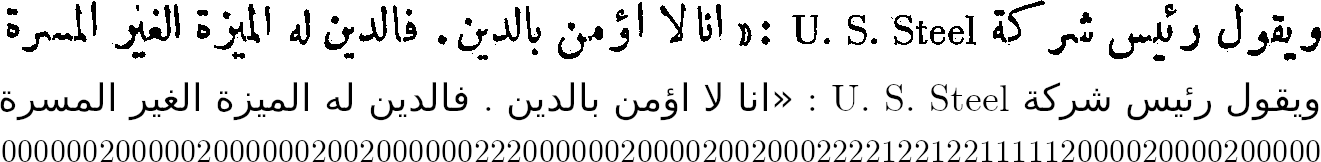
\includegraphics[width=\linewidth]{transcription.png}
        \centering
        \captionof{figure}{Modified ground truth (top: original line, middle: transcription,\\ bottom: assigned script classes)}
        \label{fig:read_transcription}
\end{figure}

Script classes are ISO 15924 codes determined through each code point's Unicode
script property\footnote{ISO 15924 includes separate identifiers for Antiqua
and Fraktur texts and similarly visually distinct calligraphic hands for Syriac
which are subsumed as Latin and Syriac in the Unicode database.} As there are
graphemes that occur in multiple scripts, chiefly numerals and punctuation, we
retain both the common and inherited properties. Merging these during
post-processing based on their surrounding script increases robustness when
classifying non-body text such as page numbers and tables, compared to fusing
them beforehand. Bidirectional text is dealt with by rearranging the target
sequence into display order using the Unicode BiDi algorithm before script
assignment.

Apart from the mentioned merging step, two additional post-processing steps are
performed. The first substitutes all individual runs of a line with the whole
line if only a single script remains after common/inherited merging. The second
stems from the observation that often only a subset of scripts the detection
network is trained on occur in any document. A whitelist is added, merging
runs of non-included scripts into the surrounding context after filtering for
common confusions (Arabic-Syriac and Latin-Fraktur).

\subsection{Emphasis Recognition}
\label{sec:emph}

We evaluated two methods of encoding two common text emphasis methods for
recognition by a RNN. Initially, italicized and text components with increased
letter spacing were marked up with special start and stop markers and the model
was trained to produce these markers. While the results of the training were
promising, obtaining the amount of training data needed to reliably place both
markers was infeasible for our target documents. Creating separate labels for
italicized/spaced graphemes and training for these, remedied the marker
placement issue with a sufficiently small amount of training data.

\begin{wrapfigure}{r}{4cm}
        \center
        \vspace{1cm}
        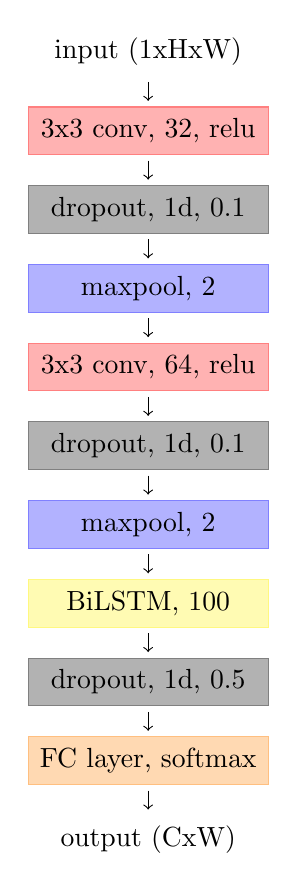
\begin{tikzpicture}[node distance = 1cm]
        \tikzset{
          base/.style={draw, align=center, minimum height=4ex, rectangle, text centered},
          proc/.style={base, draw=white, rectangle, text width=8em},
          conv/.style={proc, draw=red!50, fill=red!30},
          maxp/.style={proc, draw=blue!50, fill=blue!30},
          drop/.style={proc, draw=black!50, fill=black!30},
          lstm/.style={proc, draw=yellow!50, fill=yellow!30},
          soft/.style={proc, draw=orange!50, fill=orange!30},
          line/.style={draw, shorten <= 2pt, shorten >= 2pt, ->}
        }
        \node [proc] (input) {input (1xHxW)};
        \node [proc, conv, below of=input] (conv1) {3x3 conv, 32, relu};
        \node [proc, drop, below of=conv1] (drop1) {dropout, 1d, 0.1};
        \node [proc, maxp, below of=drop1] (maxp1) {maxpool, 2};
        \node [proc, conv, below of=maxp1] (conv2) {3x3 conv, 64, relu};
        \node [proc, drop, below of=conv2] (drop2) {dropout, 1d, 0.1};
        \node [proc, maxp, below of=drop2] (maxp2) {maxpool, 2};
        \node [proc, lstm, below of=maxp2] (lstm1) {BiLSTM, 100};
        \node [proc, drop, below of=lstm1] (drop3) {dropout, 1d, 0.5};
        \node [proc, soft, below of=drop3] (softm) {FC layer, softmax};
        \node [proc, below of=softm] (output) {output (CxW)};

        \path [line] (input) -- (conv1);
        \path [line] (conv1) -- (drop1);
        \path [line] (drop1) -- (maxp1);
        \path [line] (maxp1) -- (conv2);
        \path [line] (conv2) -- (drop2);
        \path [line] (drop2) -- (maxp2);
        \path [line] (maxp2) -- (lstm1);
        \path [line] (lstm1) -- (drop3);
        \path [line] (drop3) -- (softm);
        \path [line] (softm) -- (output);

        \end{tikzpicture}
        \captionof{figure}{Network architecture ($H$: sequence height, $W$: sequence length, $C$: alphabet size)}
        \label{fig:read_arch}
\end{wrapfigure}



Separate alphabets for emphasized text components increase model size and
execution time, tripling the size of the final fully connected layer. This
large increase in possible output labels also seems to preclude fine-tuning
base models by resizing the final linear projection of the network.

\subsection{Architecture}


Both the script detection and emphasis recognition share a common network
architecture of bidirectional Long short-term memory RNN blocks trained with
Connectionist Temporal Classification loss and single-sample stochastic
gradient descent with momentum (learning rate: 0.0001, momentum: 0.9). Early
stopping is used to terminate training. The system is implemented as part of
the kraken OCR engine.

The networks operate on binarized whole lines. Baselines and line height are
normalized using a slightly modified version of the centerline normalizer
implemented in the OCRopus system.

\section{Results}

The script detection and emphasis recognition were evaluated as part of
Bibliotheca Arabica which aims to gain new insights into Arabic literature from
1150 to 1850 CE by analysing the ways of production, transmission, and
reception of texts. The basis of this research are \textasciitilde 500 library
manuscript catalogs which are usually multilingual and employ structured text
emphasis as semantic markup.

\subsection{Dataset}

\begin{wrapfigure}{o}{0.7\textwidth}
	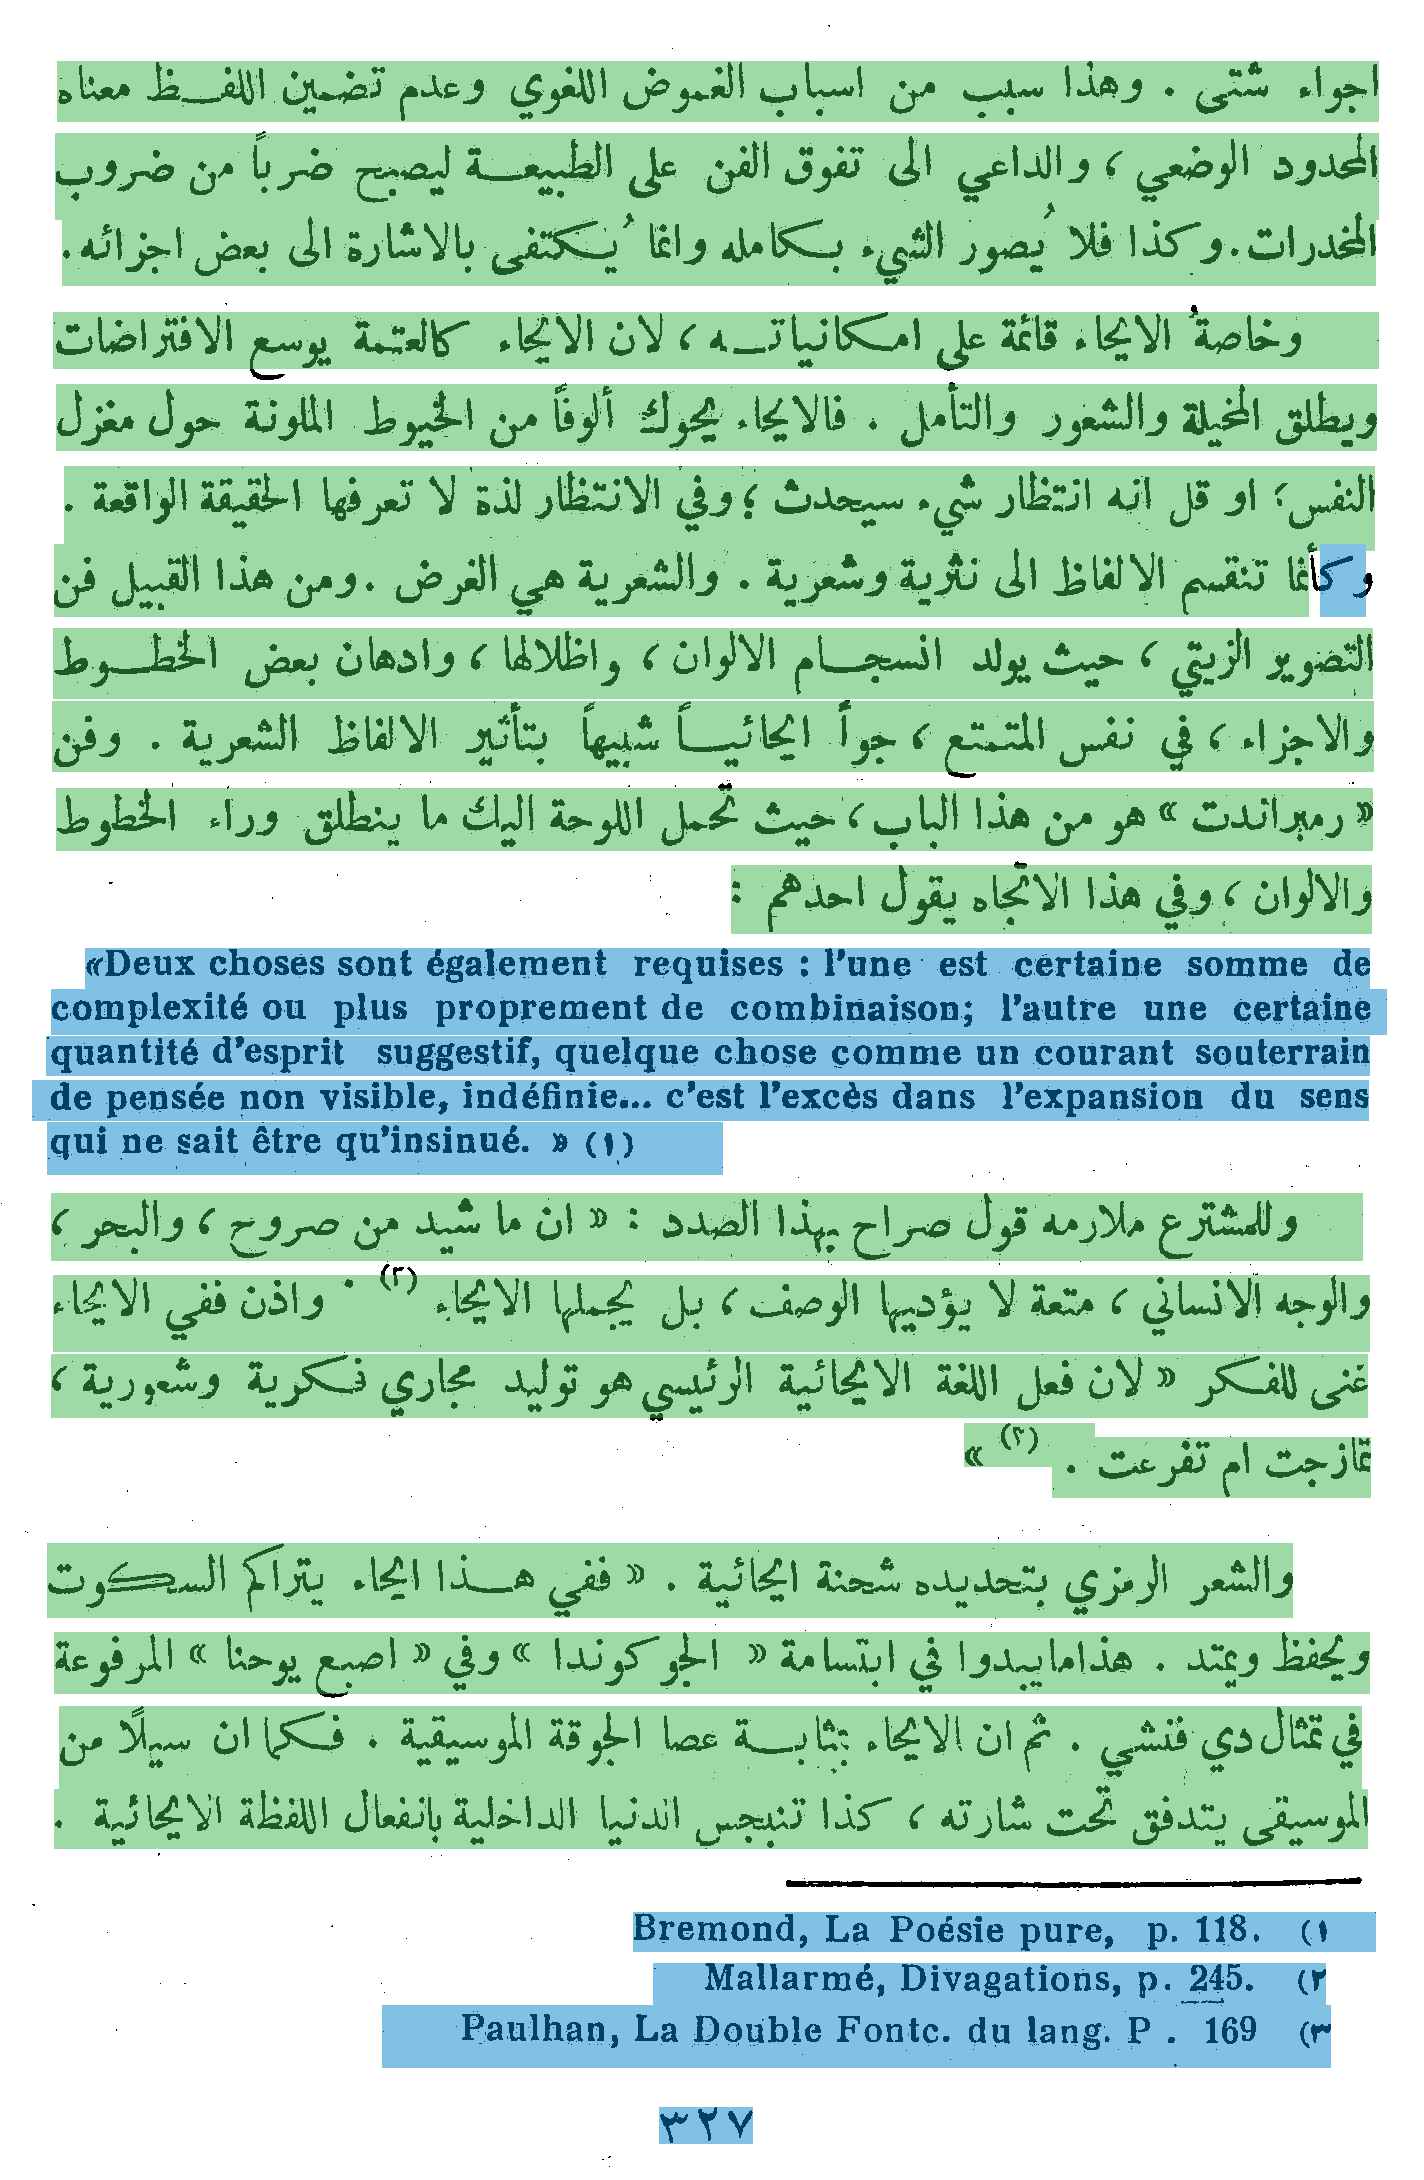
\includegraphics[width=0.68\textwidth]{high.png}
	\caption{Script recognition on French-Arabic sample page}
	\label{fig:read_high}
\end{wrapfigure}
We repurposed publicly available non-synthetic training data for recognition
models to build a corpus of 76000 script-annotated line images containing
Arabic, Cyrillic, polytonic Greek, Hebrew, Latin, Fraktur, and (western) Syriac
text. The majority of text lines contain only a single non-common script
although there are mixed lines for all scripts in the corpus. The exact
distribution of code points is shown in figure~\ref{table:points}. 760 randomly
selected lines are separated from the corpus as a test set.

Emphasis recognition was evaluated on an English and romanized Arabic catalog
using emphasis described in \ref{sec:emph} with 350 transcribed lines. An
additional fifty line tran\-scriptions were used as a test set. Over\-all 220 lines
contain some kind of text emphasis. It is representative of a large number of
catalogs in purview of Bibliotheca Arabica.

\begin{figure}
\centering
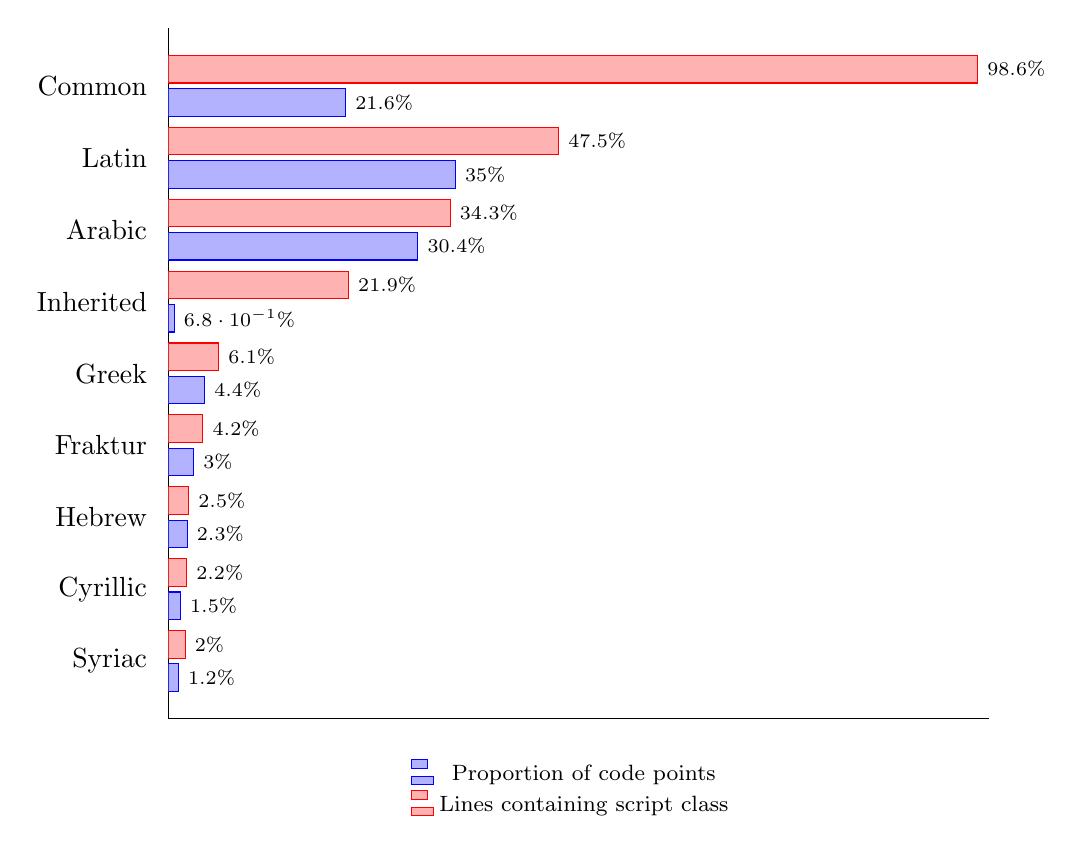
\begin{tikzpicture}
  \begin{axis}[
        axis lines*=left,
        xbar,
        width=12cm,
        xlabel={},
        xmin=0,
        xmax=1.0,
        point meta={x*100},
        ytick style={draw=none},
        xtick=\empty,
        every axis plot/.append style={fill},
        nodes near coords={\pgfmathprintnumber[precision=1]\pgfplotspointmeta\%},
        every node near coord/.append style={black, font=\scriptsize},
        nodes near coords align={horizontal},
        legend style={font=\footnotesize, draw=none, at={(0.7,-0.05)}},
        symbolic y coords={Syriac, Cyrillic, Hebrew, Fraktur, Greek, Inherited, Arabic, Latin, Common}]
          \addplot coordinates {
                (0.3496183599324223,Latin)
                (0.30396431853540445,Arabic)
                (0.21576513077364237,Common)
                (0.04403431641055621,Greek)
                (0.030492127736907817,Fraktur)
                (0.022775620241433387,Hebrew)
                (0.014548438658383681,Cyrillic)
                (0.012010166410922564,Syriac)
                (0.006791521300327209,Inherited)
        };

          \addplot coordinates {
                (0.4754016646187374,Latin)
                (0.34335659471866087,Arabic)
                (0.9863213780631999,Common)
                (0.06099738019613753,Greek)
                (0.04194004590452786,Fraktur)
                (0.02455196717130735,Hebrew)
                (0.022071267938701226,Cyrillic)
                (0.020309275960401548,Syriac)
                (0.21936800129830988,Inherited)
        };
        \legend{{Proportion of code points}, {Lines containing script class}}
  \end{axis}
\end{tikzpicture}
\caption{Script detection training data distribution}
\label{table:points}
\end{figure}

\subsection{Script Detection}

The fully trained network yielded a character accuracy of 94.62\% on the test
set. Output for a French-Arabic bilingual sample page can be seen in
\ref{fig:read_high}. The misclassification of Eastern Arabic numerals as Latin
text is caused by the transcription as Latin Arabic numerals in the ground
truth.

\subsection{Emphasis Recognition}

The average character accuracy of the trained model over 10 runs is 99.3\%
($\sigma=0.16$) with 95.38\% on cursive and text with increased spacing
($\sigma=1.46$). When using only emphasized text accuracy as the stopping
criterium mean accuracy rises to 99.03\% ($\sigma=0.28$).
